% !TEX TS-program = xelatex
% !TEX encoding = UTF-8 Unicode
% !Mode:: "TeX:UTF-8"

%This file contains the LaTeX code of my laboratory report for my ICS II course.
%Author: 张作柏/Zuobai Zhang <17300240035@fudan.edu.cn>

% This is a simple template for a LaTeX document using the "article" class.
% See "book", "report", "letter" for other types of document.

\documentclass[12pt]{article} % use larger type; default would be 10pt

\usepackage[utf8]{inputenc} % set input encoding (not needed with XeLaTeX)

%%% Examples of Article customizations
% These packages are optional, depending whether you want the features they provide.
% See the LaTeX Companion or other references for full information.

%%% PAGE DIMENSIONS
\usepackage[top=1.05in, bottom=0.95in, left=0.90in, right=1.10in]{geometry}
%\usepackage{geometry} % to change the page dimensions
\geometry{a4paper} % or letterpaper (US) or a5paper or....
% \geometry{margin=2in} % for example, change the margins to 2 inches all round
% \geometry{landscape} % set up the page for landscape
%   read geometry.pdf for detailed page layout information

\usepackage{graphicx} % support the \includegraphics command and options

% \usepackage[parfill]{parskip} % Activate to begin paragraphs with an empty line rather than an indent

%%% PACKAGES
\usepackage{booktabs} % for much better looking tables
\usepackage{array} % for better arrays (eg matrices) in maths
\usepackage{paralist} % very flexible & customisable lists (eg. enumerate/itemize, etc.)
\usepackage{verbatim} % adds environment for commenting out blocks of text & for better verbatim
\usepackage{subfig} % make it possible to include more than one captioned figure/table in a single float
% These packages are all incorporated in the memoir class to one degree or another...

%%% HEADERS & FOOTERS
\usepackage{fancyhdr} % This should be set AFTER setting up the page geometry
\pagestyle{fancy} % options: empty , plain , fancy
%\renewcommand{\headrulewidth}{0pt} % customise the layout...
\lhead{}\chead{}\rhead{}
\lfoot{}\cfoot{\thepage}\rfoot{}

%%% SECTION TITLE APPEARANCE
\usepackage{sectsty}
\allsectionsfont{\sffamily\mdseries\upshape} % (See the fntguide.pdf for font help)
% (This matches ConTeXt defaults)

%%% ToC (table of contents) APPEARANCE
\usepackage[nottoc,notlof,notlot]{tocbibind} % Put the bibliography in the ToC
\usepackage[titles,subfigure]{tocloft} % Alter the style of the Table of Contents
\renewcommand{\cftsecfont}{\rmfamily\mdseries\upshape}
\renewcommand{\cftsecpagefont}{\rmfamily\mdseries\upshape} % No bold!
\usepackage{titletoc}
\titlecontents{section}
              [1.5cm]
              {\bf \large}%
              {\contentslabel{1.8em}}%
              {}%
              {\titlerule*[0.5pc]{$\cdot$}\contentspage\hspace*{0.6cm}}%
		   [\vspace{0.5em}]
\titlecontents{subsection}
              [1.8cm]
              {\normalsize}%
              {\contentslabel{2.0em}}%
              {}%
              {\titlerule*[0.5pc]{$\cdot$}\contentspage\hspace*{0.6cm}}%
		   [\vspace{0.4em}]
\titlecontents{subsubsection}
              [2.1cm]
              {\small}%
              {\contentslabel{2.5em}}%
              {}%
              {\titlerule*[0.5pc]{$\cdot$}\contentspage\hspace*{0.6cm}}%
		   [\vspace{0.4em}]


\usepackage[UTF8]{ctex}
\usepackage{fancyhdr}
\usepackage{enumerate}
\usepackage{indentfirst}
\usepackage{extramarks}
\usepackage{titling}
\usepackage{xcolor}
\usepackage{fontspec}
\usepackage[CJKbookmarks=true,colorlinks,linkcolor=black]{hyperref}
\setmainfont{Times New Roman}

%%% END Article customizations

%%% The "real" document content comes below...

%\title{\textbf{Digital Logic and Computer Design Report}}
\title{\textbf{KDD Cup 2012 Track 1解题报告}}
\author{张作柏\\17300240035}
%\date{} % Activate to display a given date or no date (if empty),
         % otherwise the current date is printed 

\usepackage{amsmath}
\newcommand\calD{\mathcal{D}}
\newcommand\XX{\boldsymbol{\mathit{X}}}

\begin{document}
\begin{sloppypar}
\maketitle

\pagestyle{fancy}
\lhead{\textbf{{\thetitle}}}
\rhead{\textbf{\nouppercase{\firstleftmark}}}
\cfoot{\thepage}

\thispagestyle{empty}
\tableofcontents
\clearpage

\setcounter{page}{1}


\section{任务简介}

本次PJ我选择了KDD Cup 2012 Track 1题目\footnote{\url{https://www.kaggle.com/c/kddcup2012-track1}},其中模型主要参考了~\cite{chen2012context}一文。

\subsection{任务描述}

近年来,随着像Facebook、Twitter、腾讯微博等社交平台的发展,在线社交网络引起了广泛的关注。全中国最大的微博系统之一,腾讯微博,已经成为网络社交的重要平台。目前,腾讯微博拥有超过2亿的注册用户,每天产生四千万条信息。海量的数据引起了数据挖掘爱好者的注意,如何利用数据信息改善用户的使用体验,成为了一个十分有趣并值得研究的问题。

本任务中,我们需要根据用户的兴趣,预测他是否会关注某个对象(item)。对象可以是某个组织、个人、群体等等。最终我们要在所有备选推荐中,选择至多三个对象推荐给用户。

\subsection{数据信息}

\subsubsection{名词定义}

{\bf 对象(item):} 对象是腾讯微博中的一个用户,他可以代表组织、个人或群体。数据集中大约有六千个不同的对象。

{\bf 发微博(tweet):} 发微博是指用户可以在微博系统中发表一条信息,他的关注者会看到这条信息的提醒。

{\bf 转发(retweet):} 用户可以转发其他用户发表的信息,并在其下添加评论。

{\bf 评论(comment):} 用户可以在别人的微博下发表评论。

{\bf 关注者(follower):} 用户可以关注其他用户,若用户A关注了B,则称A是B的关注者。

\subsubsection{数据文件}

\begin{enumerate}
	\item {\bf 训练数据集rec\_log\_train.txt:} 记录了用户与对象之间的历史推荐结果。\\
	文件格式:(UserId) (ItemId) (Result) (Unix-timestamp)\\
	在Unix-timestamp的时间,系统向用户UserId推荐了物品ItemId,得到的结果为Result。Result为1,表示接受;Result为-1,表示拒绝。
	\item {\bf 测试数据集rec\_log\_test.txt:} 记录了测试集中用户与对象之间的可能推荐。\\
	文件格式同训练数据集rec\_log\_train.txt\\
	区别在于其中Result域为0,需要我们来预测。
	\item {\bf 用户信息user\_profile.txt:} 记录了用户的详细个人资料。\\
	文件格式:(UserId) (Year-of-birth) (Gender) (Number-of-tweet) (Tag-Ids) \\
	依次表示用户的Id,出生日期,性别,发表的微博数量和标签。其中,出生日期将以年份的形式给出;性别为0、1、2,分别代表未知、男性、女性;标签是由用户选择的代表个人兴趣的关键词,有的用户没有选择标签,标签的格式为:tag-id1;tag-id2;...;tag-idN,其中每个标签用正整数来表示,如果一个用户没有任何标签的话,那么他的tag-id为0。
	\item {\bf 对象数据item.txt:} 记录对象的属性,包含它所属的类别与关键词。\\
	文件格式:(ItemId) (Item-Category) (Item-Keyword) \\
	依次表示对象的Id,对象所属的类别(以“a.b.c.d”的格式给出,表示所属的子类别),Item-Keyword是从对象的个人资料中提取的关键词,以"id1;id2;...;idN"的形式给出。
	\item {\bf 用户行为user\_action.txt:} 记录了用户在微博上的行为,包括艾特、转发和评论。 \\
	文件格式:(UserId) (Action-Destination-UserId) (Number-of-at-action) (Number-of-retweet) (Number-of-comment) \\
	假如用户A转发了B的微博5次,'@'B共3次,评论6次,则相应的数据为“A B 3 5 6”。
	\item {\bf 用户关注行为user\_sns.txt:} 描述用户的关注信息。 \\
	文件格式:(Follower-userid) (Followee-userid) \\
	表示前者关注了后者。
	\item {\bf 用户关键词描述user\_key\_word.txt:} 记录了从用户的微博信息中提取的关键词。\\
	文件格式:(UserId) (Keywords) \\
	其中关键词的格式为“kw1:weight1;kw2:weight2;...kwN:weightN”。关键词是从用户的微博中提取的,可以用来预测用户的兴趣,权值表示用户对某个关键词的感兴趣程度,权值越大,越感兴趣。每个关键词都用唯一的整数表示,并与item的关键词共用一个字典。
\end{enumerate}

\subsubsection{注意事项}

以下是一些没有在题目中给出,但是我在数据处理的过程中发现的问题:
\begin{itemize}
\item 对象item的ID与用户user的ID是共用一个词典的,即每个ItemId也对应一个UserId。
\item 用户的性别并非只有0、1、2三种,还有性别为3的用户。
\item 用户填写的出生年中存在非法数据,格式不正确,不是年份的形式。
\end{itemize}

\subsection{提交格式}

原提交网站上的提交格式说明消失了,我是从别人的博客上看到的,并结合讨论区的评论和自己的一些理解,总结出的以下格式。

测试集rec\_log\_test.txt中包含了不重复的$34,910,937$对用户与对象,以及相应的推荐时间,但未给出推荐的结果。文件是按照时间顺序排序的,时间$<1,321,891,200$的记录将被用于public leaderboard,而时间$>=1,321,891,200$的记录将被用于private leaderboard的最终评测。我们的目标是预测每个集合中推荐给用户的item。

因为腾讯的默认设置是最多推荐三个item给用户,所以在每个测试集上,我们需要为每个用户推荐至多三个item,且按照顺序排序,这将在评价指标的度量中起到作用。

最终提交时,上传一个.csv文件,文件总共两列,包括UserId与ItemIds,分别表示用户的Id和推荐给他的对象Id。public leaderboard数据在前,private数据在后,分别按照用户Id升序排列,推荐的对象按照推荐顺序排序。最终提交的文件中必须恰好包含$1,340,127$行。

\subsection{评价方式}

本次比赛使用的是MAP(Mean Average Precision)作为评价指标,计算方式如下:
\begin{equation}
ap@n = \sum_{k} P(k) / (\textit{用户接受总数}),
\end{equation}
其中$P(k)$表示前$k$个物品中用户接受的个数,若物品$k$未被接受,则规定$P(k)=0$。

在该任务中,我们至多推荐三个item给用户,故$n=3$,item按顺序记为\#1,\#2,\#3。

假如用户总共接受了3个物品,分别是\#1,\#3,\#4,那么$ap@3 = (\frac{1}{1} + \frac{2}{3}) / 3 \approx 0.56$。

假如用户总共接受了4个物品,分别是\#1,\#2,\#4,那么$ap@3 = (\frac{1}{1} + \frac{2}{2}) / 3 \approx 0.67$。 

假如用户总共接受了2个物品,分别是\#1,\#3,那么$ap@3 = (\frac{1}{1} + \frac{2}{3}) / 2 \approx 0.83$。 

\subsection{为什么使用Julia?}

Julia是一种用于科学计算的新兴语言,其最大的特点是速度快,号称兼具Python的便捷性与C的速度。在本次项目中,我使用了Julia语言,一是因为想要熟悉一下这门新的语言,并在后续的研究中使用,二是因为Python的效率太低,且对于本任务并无太大用处,所以不妨使用新的Julia语言。

因为在这次的PJ中,我的训练过程是手写的,未使用自动求导的模块,所以其中涉及到大量的矩阵、向量运算。而Julia对于这些线性代数操作,支持许多快速的算法,具有与MATLAB比肩的数值分析运算能力。这也是我使用Julia的主要原因之一。


\newpage
\section{数据预处理}

本节主要介绍在数据预处理过程中使用的方法,主要方法与~\cite{chen2012context}一文相同,有一些小细节进行了改动。

\subsection{会话分析}

训练集中共有$73,209,277$个训练数据,其中涉及$1,392,873$个用户和$4,710$个对象。其中,包含$5,253,828$个正例和$67,955,449$个负例。可以看到,负例的个数远超过正例的个数,那实际上所有的负例都是有效的吗?其实不然。这些记录是从现实生活中的用户浏览记录中提取的,而实际中我们自己在浏览微博时,更多是关注于微博的内容,而不是微博的推荐内容。所以用户没有接受一个推荐,并不一定说明用户真的对这个对象不感兴趣,而有可能是因为用户并没有意识到这个推荐。因此,为了便于我们对用户的兴趣建模,我们需要先剔除一部分的噪声数据。

这里,我认为论文中的方法不是很正确,且实现后发现得到的数据与论文中给出的并不一致,所以我没有完全照搬论文中的方法。

因为每个用户的浏览习惯是不同的,这一点主要体现在浏览时长上。对于每个用户,我们对将所有对他的推荐,按时间顺序排序,然后计算相邻两个推荐时刻之间的间隔,即
\begin{equation}
	\Delta t_s = t_{s+1} - t_s,
\end{equation}
其中,$t_s$和$t_{s+1}$分别对应第$s$个推荐时刻和第$s+1$个推荐时刻。这里需要注意,因为会有对象在同一时刻被推荐,所以这里要计算相邻两个时刻,而非相邻两个对象的时间间隔。

我们需要将用户的推荐记录划分为若干个时间段,时间段之间是互相独立的,因此需要先计算一个阈值$\tau$,当相邻时间间隔大于等于$\tau$时,则说明可以将两边划分为两个互不影响的时间段。那么,为了避免过大的时间间隔的影响,我们在确定阈值时,只考虑相邻间隔不超过一个小时的数值,即如果$\Delta t_s<3600$的话,我们将其记为$\ddot{\Delta t_s}$,只考虑这一部分时间间隔。对所有的时间间隔取平均,得到阈值
\begin{equation}
\tau = \frac{1}{2} \times (\tau_0 + \frac{\sum_{s}\ddot{\Delta t_s}}{|\ddot{\Delta t}|}).
\end{equation}
其中,$|\ddot{\Delta t}|$表示不超过一小时的时间间隔个数。取$\tau_0=90$,计算得到阈值$\tau$,对于大于$\tau$的时间间隔,我们把它分为两个时间段。

现在,我们将第$k$个时间段中的样本集合记为$\Phi_k$,其中的正样本记为$\Phi^+_k$。记出现最早的正样本的下标记为$\sigma_-$,最晚出现的记为$\sigma_+$,那么对于下标为$\sigma_s$的样本,我们进行如下过滤:
\begin{enumerate}
	\item 若该时间段出现的正样本过多,则说明可能这是噪声数据,将这个时间段中的数据全部剔除,即只选择$0< \frac{|\Phi^+_k|}{|\Phi_k|} \le \epsilon$的时间段,其中取$\epsilon=0.86$。
	\item 我们在下标区间$\sigma_--\pi_-$到$\sigma_++\pi_+$中选取样本,即样本$\sigma_s$需要满足$\sigma_--\pi_-\le\sigma_s\le\sigma_++\pi_+$。这一限制是基于假设:用户可能在意识到第一个正样本之前,一直没有关注到推荐,可能在接受最后一个正样本之后,就没有再留意推荐信息。这里,为了减少样本数量,提高训练效率,我们取$\pi_+=\pi_-=1$。
\end{enumerate}

最后,经过数据清洗,我们得到$3,794,928$个正例和$11,193,905$个负例,总共约一千五百万的训练数据,数据量缩减五倍,这大大提升了训练的效率。

\subsection{成对训练}

不同于寻常的二分类问题,在这一问题中,我们需要对所有的推荐物品进行排序,这更像是一个学习排名的问题~\cite{liu2009learning}。实践证明~\cite{furnkranz2003pairwise}~\cite{rendle2014improving}~\cite{sharma2013pairwise},以分类问题中常使用的MSE(Mean Square Error)作为目标函数进行训练的效果不是很好。在这一问题中,我们使用更加适合排名问题的成对训练方法。这一方法在推荐系统中的应用比较广泛,且非常适合排名问题。

成对训练的基本思路是,将一个正例与一个负例组合,通过训练使得正例的概率尽可能的高于负例的概率。如何构造成对的组合呢?对于每个用户,因为负例的数量较多,所以我们对于它的每一个负例,随机挑选一个正例与它匹配,最终,我们将得到$11,193,905$个训练样本。


\newpage
\section{用户兴趣模型}

\subsection{基本模型}

\subsection{成对训练}

\subsection{年龄、性别因素}

\subsection{间接反馈信息}

\subsection{关键词、标签信息}

\subsection{用户、物品信息}


\newpage
\section{用户行为模型}

\subsection{时间度量}

\subsection{概率预测}


\newpage
\section{集成学习AdaBoost}

本节中我们将组合方法融入模型中,组合分类器(ensemble)是一个复合模型,由多个分类器组合而成,个体分类器投票,组合分类器基于投票返回类标号预测。组合分类器往往比成员分类器更准确。

\subsection{模型原理}

自适应提升算法(Adaptive Boosting)是一种机器学习算法,由Yoav Freund和Robert Schapire于1997年首次提出~\cite{freund1997decision}。其基本思想是:前一个分类器分错的样本会被用来训练下一个分类器,相对于大多数其他学习算法而言,不容易出现过拟合现象。

AdaBoost可被应用于人脸识别~\cite{wu2004fast},网络入侵检测~\cite{hu2008adaboost},预测蛋白质结构~\cite{niu2006predicting}等机器学习问题。此外,它还可以用于处理不平衡数据~\cite{viola2002fast},非常适合处理我们这道题中正样本较少的情况。

关于AdaBoost的原理可参考教材~\cite{han2011data}第380页和这篇博客~\footnote{\url{https://www.cnblogs.com/pinard/p/6133937.html}}。图~\ref{fig:AdaBoost}描述了AdaBoost的基本过程~\footnote{图源自\url{https://www.datacamp.com/community/tutorials/adaboost-classifier-python}}。其基本原理如下:

给定数据集$\calD$,它包含$d$个类标记的元组$(\XX_1, y_1), (\XX_2, y_2), \cdots, (\XX_d, y_d)$,其中$y_i$是元组$\XX_i$的类别标号。初始时,AdaBoost对每个训练元组赋予相等的权重$1/d$。为了组合$k$个基分类器,我们将进行$k$轮迭代。每次迭代过程如下:
\begin{enumerate}
\item 按训练元组的权重从$\calD$进行有放回抽样,得到训练集$\calD_i$。
\item 使用训练集$\calD_i$训练分类器$M_i$。
\item 计算分类器$M_i$在$\calD_i$上的分类误差。若误差大于$0.5$,则重新训练该模型。
\item 对于每个分类正确的元组,调整其权重,将其权重乘以$\frac{error(M_i)}{1 - error(M_i)}$,其中$error(M_i)$表示分类器$M_i$的分类误差。
\item 规范化训练元组的权重。
\end{enumerate}

当使用组合分类器对新元组$\XX$分类时,设置模型$M_i$的投票权重为$\log\frac{1-error(M_i)}{error(M_i)}$,最后返回最大权重的类。

\begin{figure}[htbp]
	\centering
	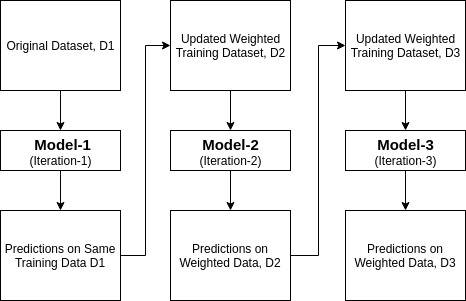
\includegraphics[width=0.85\linewidth]{figure/AdaBoost.jpg}
	\caption{AdaBoost流程}
	\label{fig:AdaBoost}
\end{figure}

\subsection{训练方法}

不同于普通的分类问题,本问题是一个Learning to Rank的模型,不能简单地套用AdaBoost算法。且我们在训练时使用的是pairwise training方法,而在预测时需要对所有推荐物品排序,这其中的差异使得AdaBoost的应用并不方便。

我做的一个尝试是:在训练时仍采用抽样-pairwise training-更新权重的方法。pairwise training中每个元组可视为一个二分类问题,目标是使得正样本的出现概率高于负样本。计算分类器误差时,若某一元组的概率大于$0.5$,则将其视为正确分类的样本。在分类时,将$K$个分类器的权重进行加权平均,后比较所有物品的权重,取其中最大的三个作为最终的推荐结果。该方法最终取得了比较好的效果。

\paragraph{参数设置}
受系统内存大小限制,我们无法使用较多的模型进行组合,故仅设置模型数量$K$为$5$。对于每个模型,设置其参数维度$d=90$,学习率为$0.00025$。每次训练的过程中,从整个训练样本中有放回的抽样$10,000,000$个样本。整个训练过程在服务器上持续了一个星期,也足以说明这个问题的规模之大。


\newpage
\section{结果评估}

\subsection{测试模块}

\subsection{测试结果}

\newpage
\section{结论}



\newpage
\bibliographystyle{unsrt} 
\bibliography{PJ}


\section*{致谢}

\addcontentsline{toc}{section}{致谢}

感谢张宇恒同学与我交流论文复现中的细节!


\end{sloppypar}
\end{document}
